\chapter{Архитектура Faster R-CNN} \label{appendix1}							% 
%\addcontentsline{toc}{chapter}{Архитектура Faster R-CNN}	% Добавляем его в оглавление

% TODO теряются картинки
\begin{figure}
	\begin{center}
	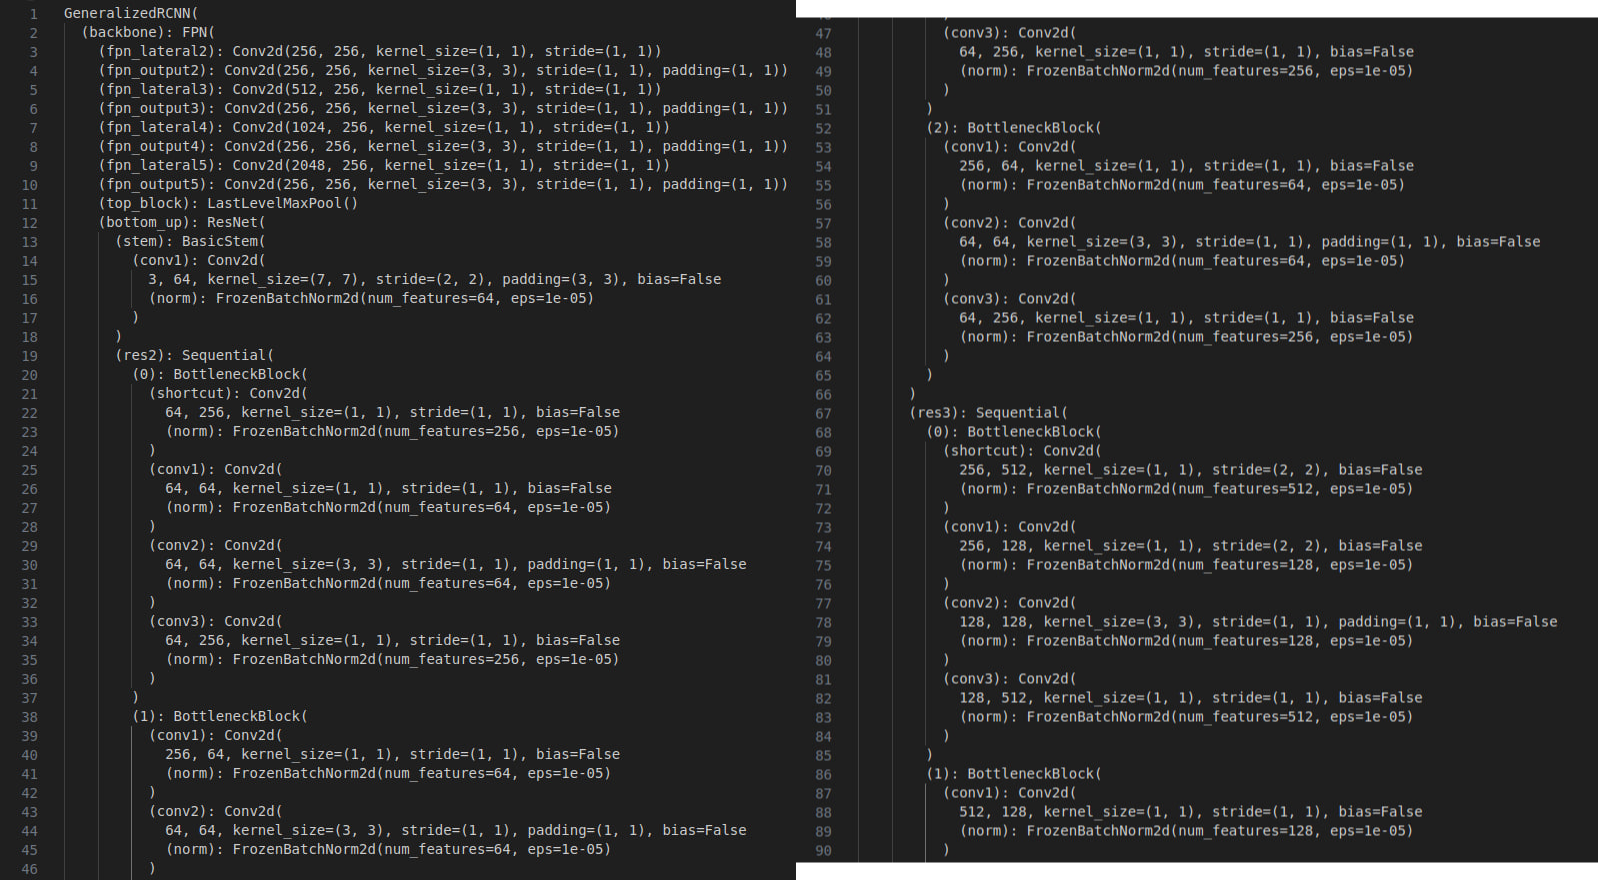
\includegraphics [scale=0.27]{my_folder/images/arch12}
	\label{fig:arch12}
	\end{center}
	\caption{Архитектура Faster R-CNN (1)}
\end{figure}
\begin{figure}
	\begin{center}
	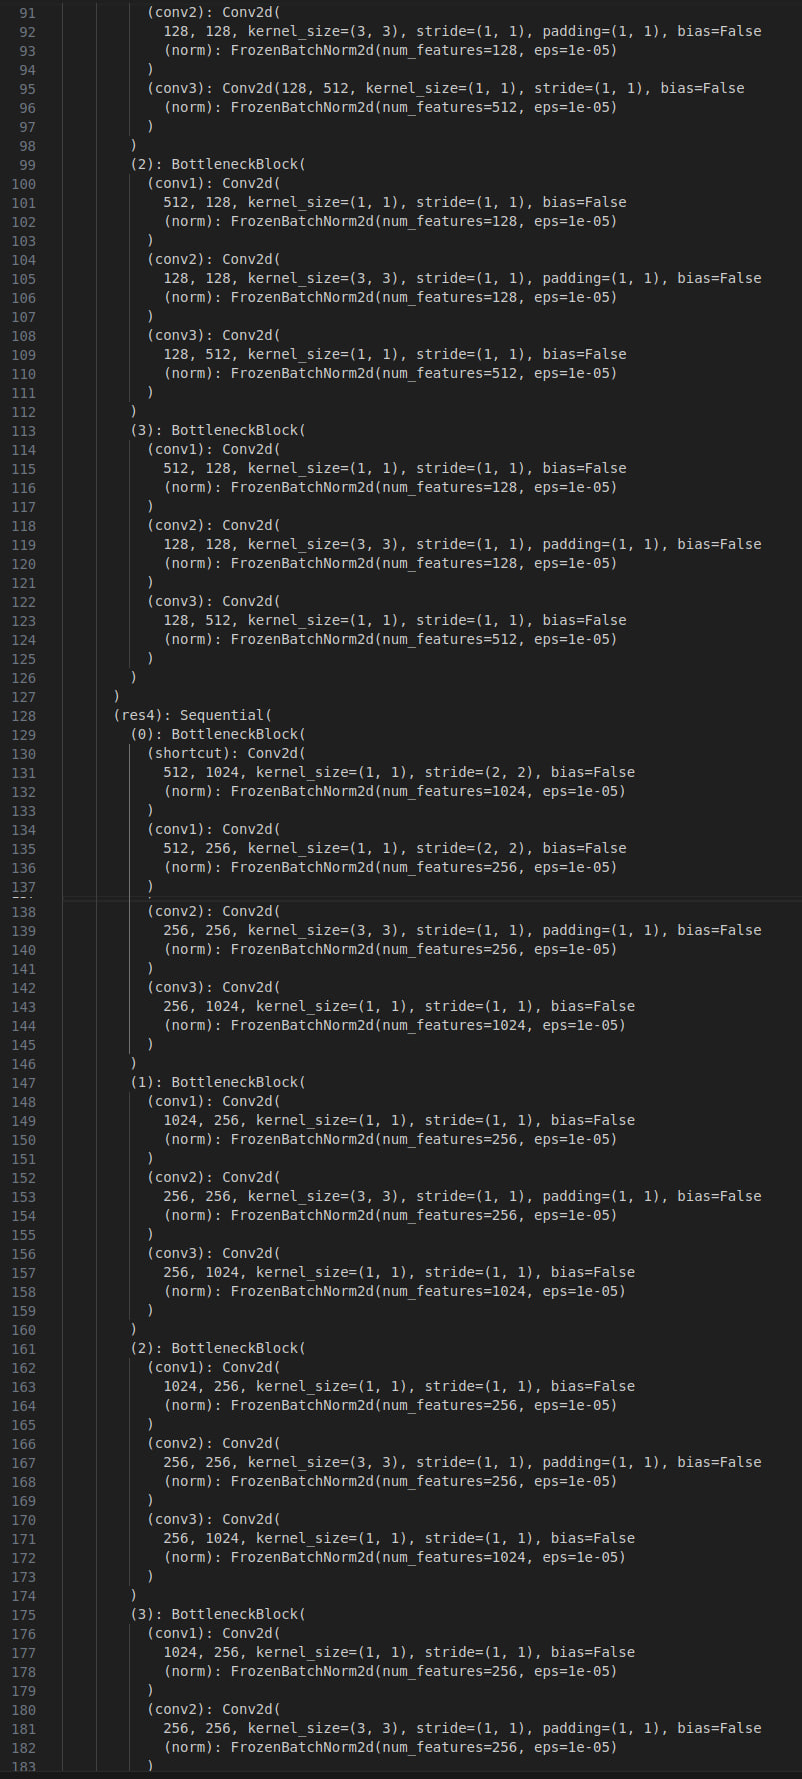
\includegraphics [scale=0.26]{my_folder/images/arch34}
	\label{fig:arch34}
	\end{center}
	\caption{Архитектура Faster R-CNN (2)}
\end{figure}
\begin{figure}
    \begin{center}
	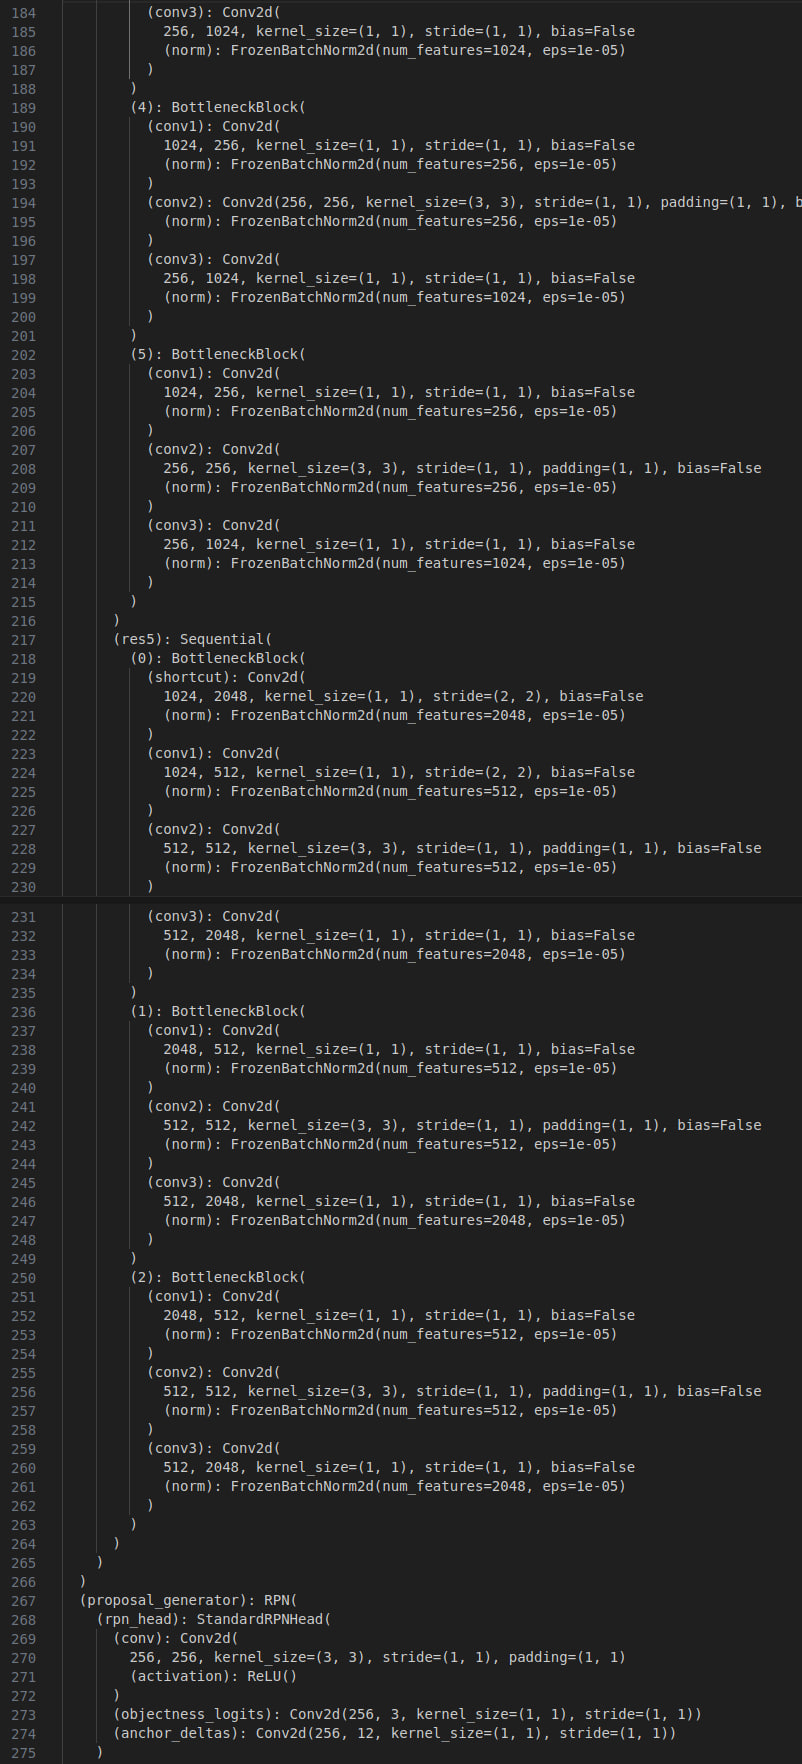
\includegraphics [scale=0.26]{my_folder/images/arch56}
	\label{fig:arch56}
	\end{center}
	\caption{Архитектура Faster R-CNN (3)}
\end{figure}
\begin{figure}
	\begin{center}
	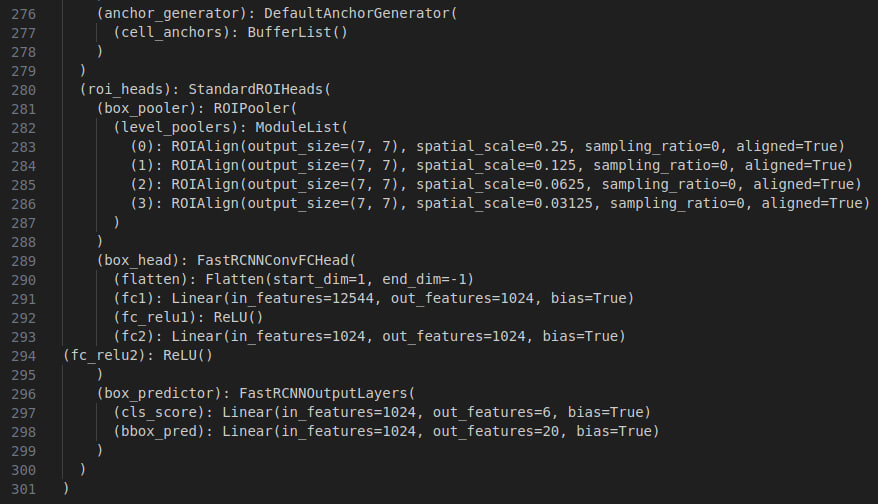
\includegraphics [scale=0.6]{my_folder/images/arch7}
	\caption{Архитектура Faster R-CNN (4)}
	\end{center}
	\label{fig:arch7}
\end{figure}
\FloatBarrier
%
%% В случае, когда таблица (рисунок) размещаются на последней странице, для переноса названия приложения на новую строку используем:
%\NewPage % начать новое приложение с новой страницы 